\documentclass[11pt,letterpaper]{article}

\usepackage[margin=0.9in]{geometry}
\usepackage{graphicx}
\usepackage{amsmath}
\usepackage{booktabs}
\usepackage{enumitem}
\usepackage{microtype}
\usepackage[ruled,linesnumbered]{algorithm2e}
\usepackage[hidelinks]{hyperref}

\setlist[itemize]{leftmargin=1.4em,itemsep=0.2em,topsep=0.3em}
\newcommand{\dataset}{\textit{Scoba 12}}

\title{Skeleton-Based Analysis of Three-Dimensional Melt Networks\\
\large Technical Report for the CSE Master's Project}
\author{Yuan Liu\\
Washington University in St. Louis\\
Advisor: Professor Tao Ju}
\date{Project completed December 2022\\
Report revised September 2026 for clarity and archival presentation}

\begin{document}
\maketitle

\begin{abstract}
Coordination-number distributions summarize how melt tubules connect at junctions in three-dimensional rock microstructures. Manual annotation can be accurate but is slow, while automated estimates are sensitive to imaging noise, ambiguous sheet-like regions, and closely spaced junctions. This project develops a skeleton-based pipeline that preprocesses a binary melt volume, extracts a topology-preserving skeleton, filters ambiguous regions, merges nearby junction candidates, and computes coordination numbers from the resulting graph. The project-specific contributions are the graph-based collection of junction candidates, a geometry-aware junction-merging procedure, and coordination-number estimation. Experiments on the \dataset{} volume and a manually labeled subvolume show that the method recovers the overall distribution but still overcounts three-way junctions and undercounts four-way junctions. The report documents the method, evaluates the available evidence conservatively, and identifies concrete failure modes and directions for a more rigorous benchmark.
\end{abstract}

\section{Project Scope and Contributions}

This master's project was conducted under the supervision of Professor Tao Ju in collaboration with Professor Philip Skemer of the Department of Earth and Planetary Sciences at Washington University in St. Louis. The three-dimensional microtomography data were provided by Professor Skemer's laboratory.

The complete pipeline combines established geometry-processing components with project-specific graph analysis:
\begin{itemize}
    \item Existing components perform morphological preprocessing and skeleton extraction using Voxel Cores and Erosion Thickness \cite{voxelcore,erosionthickness}.
    \item This project collects candidate junctions from the skeleton graph, removes candidates inside ambiguous regions, merges candidates that represent the same physical junction, and estimates the coordination-number distribution.
    \item The implementation and archival project materials are available in the \href{https://github.com/HiveYuan/Skeleton_Analysis_of_Melt_Network}{project repository}.
\end{itemize}

This document is a master's research technical report, not a peer-reviewed publication.

\section{Background and Motivation}

\subsection{Melt networks}

Partial melting occurs when only part of a solid rock melts. Beneath mid-ocean ridges, adiabatic decompression produces partial melt in ascending mantle peridotite. The buoyant melt migrates through the mantle and contributes to the formation of oceanic crust. In a partially molten material, melt may form connected tubules and junctions or isolated pockets, depending on interfacial energy and local microstructure \cite{skemerMelt}.

Figure~\ref{fig:volumes} shows the full \dataset{} binary volume and a smaller subvolume used in this project.

\begin{figure}[htbp]
    \centering
    \begin{minipage}[t]{0.48\textwidth}
        \centering
        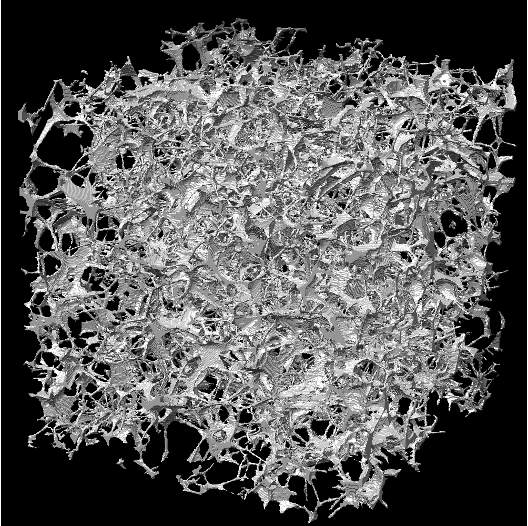
\includegraphics[width=\linewidth]{images/melt_network.png}
        \small (a) Full volume: $500^3$ voxels.
    \end{minipage}\hfill
    \begin{minipage}[t]{0.48\textwidth}
        \centering
        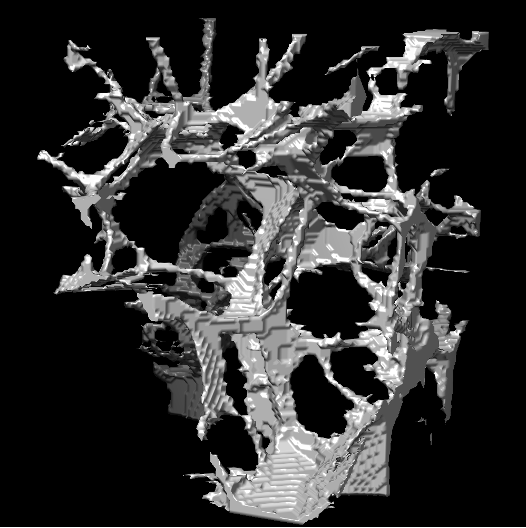
\includegraphics[width=\linewidth]{images/small_chunk.png}
        \small (b) Evaluation subvolume: $112\times118\times142$ voxels.
    \end{minipage}
    \caption{Two views of the \dataset{} melt-network data.}
    \label{fig:volumes}
\end{figure}

\subsection{Coordination number}

A melt junction is a location where multiple tubules meet. Its \emph{coordination number} (CN) is the number of incident tubules. For example, a junction connected to three tubules has CN~$=3$. A coordination-number distribution records the relative frequency of junctions at each CN and provides a compact description of network topology. Correctly estimating this distribution matters because melt-network topology influences permeability and other transport properties \cite{skemerMelt}.

\begin{figure}[htbp]
    \centering
    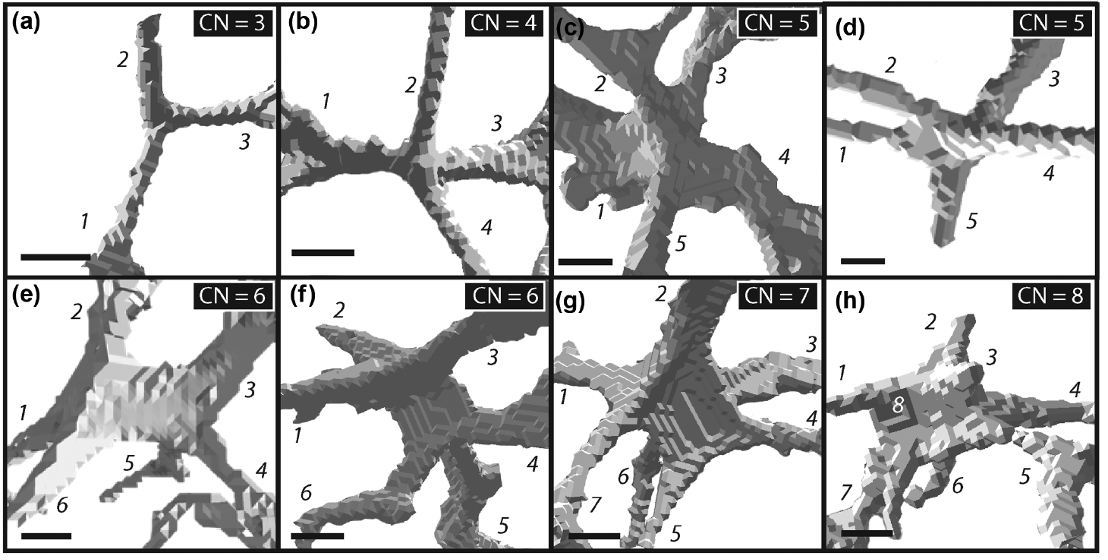
\includegraphics[width=0.72\textwidth]{images/Different_CN.png}
    \caption{Examples of melt-network junctions with different coordination numbers.}
    \label{fig:different-cn}
\end{figure}

\subsection{Problem statement}

Manual CN annotation is labor-intensive: a $500^3$ volume can require weeks of inspection. Automated methods are much faster, but errors in topology extraction can change the estimated distribution. This project therefore asks:

\begin{quote}
Can a geometry- and graph-based pipeline estimate the coordination-number distribution of a three-dimensional melt network while reducing the manual effort required for analysis?
\end{quote}

The main technical difficulty is that the input is not ideal. Measurement noise creates small holes and broken branches; sheet-like or unusually thick regions do not behave like ordinary junctions; and one physical junction may appear as several nearby vertices after skeletonization.

\section{Method}

\subsection{Pipeline overview}

The method transforms a binary volume into a graph and then into a coordination-number histogram:

\begin{enumerate}[leftmargin=1.7em,itemsep=0.25em]
    \item Dilate the binary melt volume to reduce small holes and short discontinuities.
    \item Extract a skeleton with Voxel Cores and Erosion Thickness \cite{voxelcore,erosionthickness}.
    \item Use a second Erosion Thickness configuration to identify ambiguous thick or sheet-like regions.
    \item Collect skeleton vertices with degree greater than two and discard candidates inside ambiguous regions.
    \item Merge connected junction candidates that likely represent the same physical junction.
    \item Compute each remaining junction's graph degree and aggregate the CN distribution.
\end{enumerate}

\begin{figure}[htbp]
    \centering
    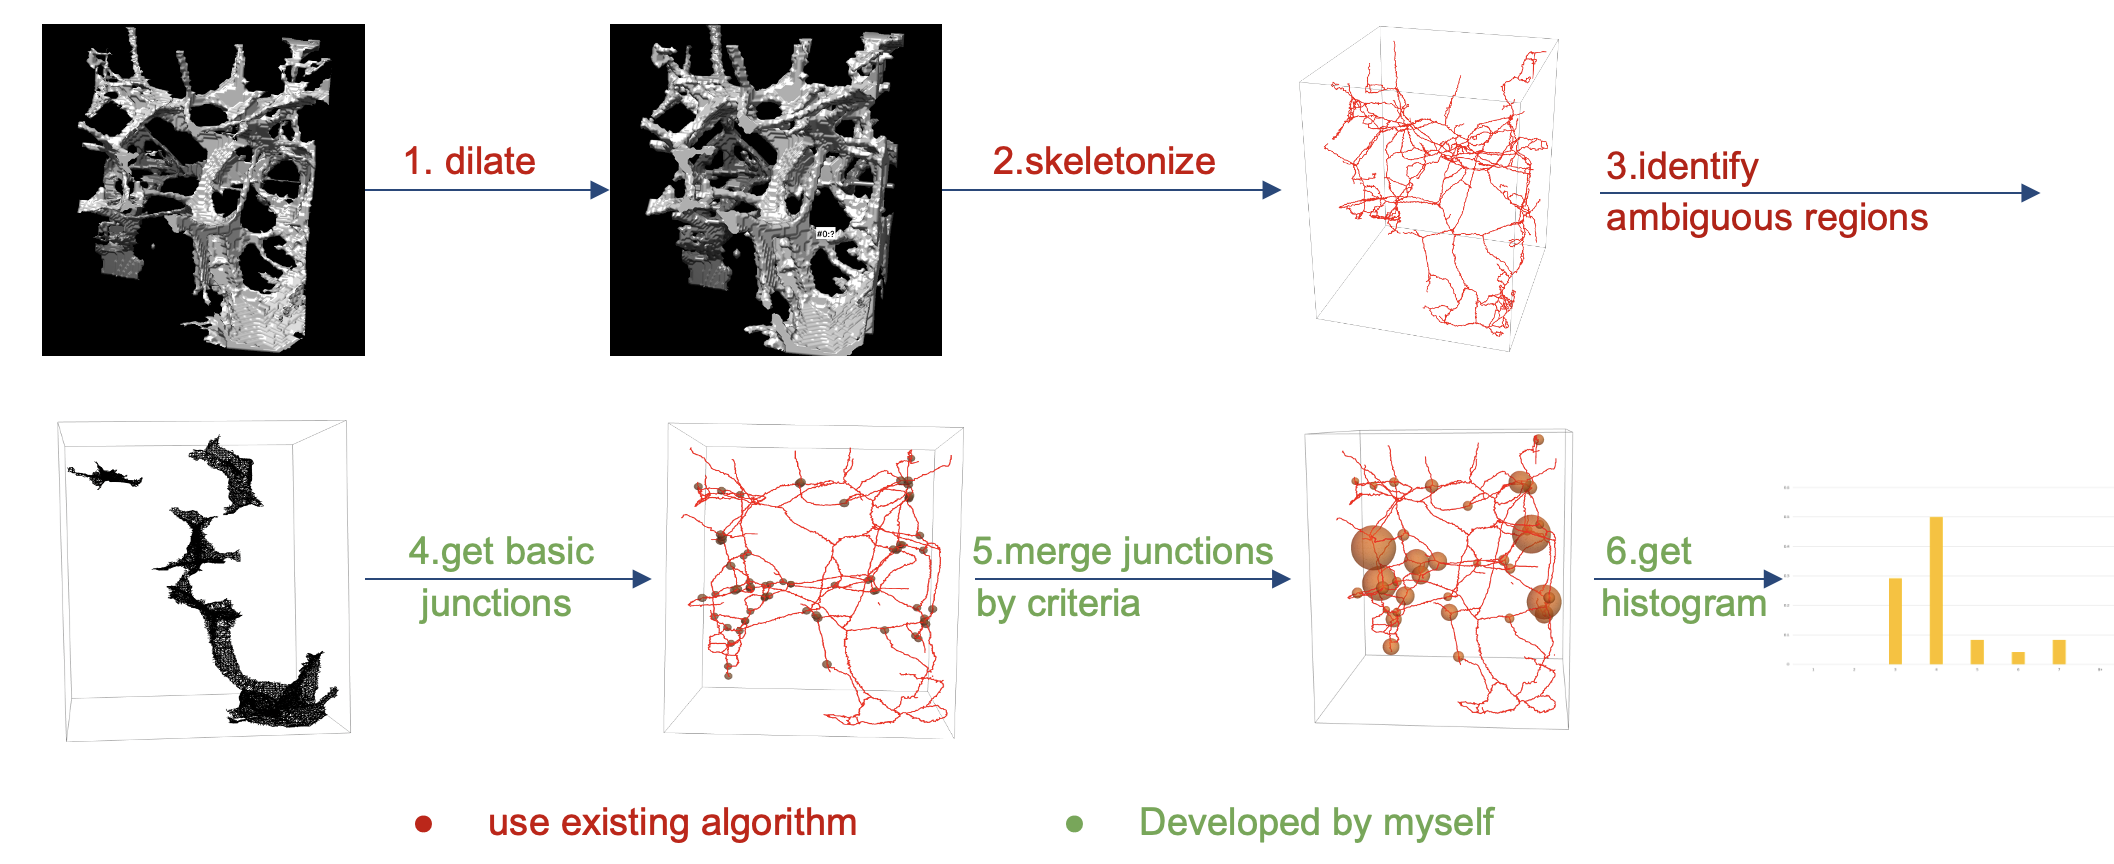
\includegraphics[width=0.95\textwidth]{images/pipeline.png}
    \caption{Processing pipeline from a binary melt volume to a coordination-number distribution.}
    \label{fig:pipeline}
\end{figure}

\subsection{Morphological preprocessing}

Dilation expands the foreground boundary with a local structuring element. In this application, it fills many small holes and lengthens short broken branches while preserving larger cavities that are more likely to be part of the network topology. The operation is a practical noise-reduction step rather than a guarantee that all defects are corrected.

\begin{figure}[htbp]
    \centering
    \begin{minipage}[t]{0.48\textwidth}
        \centering
        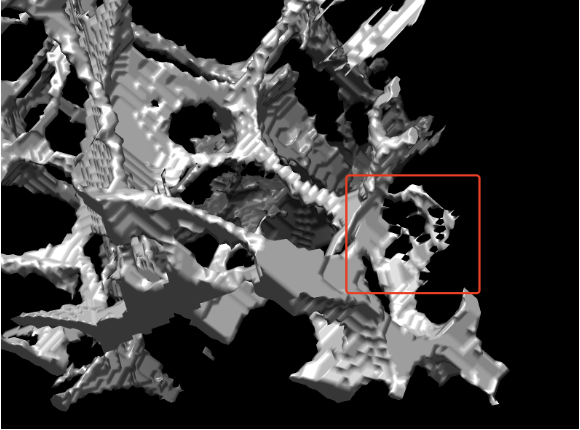
\includegraphics[width=\linewidth]{images/tiny_holes.png}
        \small (a) Input with small holes.
    \end{minipage}\hfill
    \begin{minipage}[t]{0.42\textwidth}
        \centering
        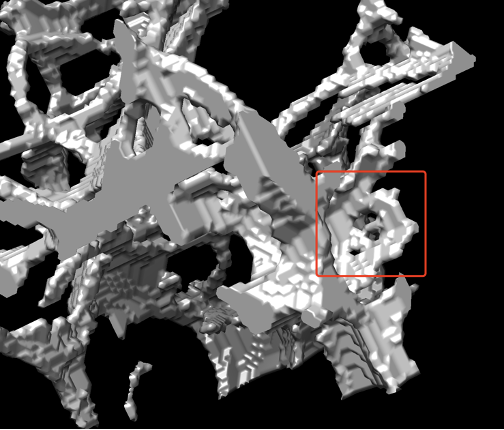
\includegraphics[width=\linewidth]{images/dilate_hole.png}
        \small (b) Volume after dilation.
    \end{minipage}
    \caption{Dilation suppresses small voids that would otherwise introduce spurious skeleton branches.}
    \label{fig:dilation}
\end{figure}

\subsection{Skeleton extraction and ambiguous-region filtering}

The Voxel Core method provides a robust approximation of the three-dimensional medial axis, and Erosion Thickness helps distinguish prominent structure from boundary noise \cite{voxelcore,erosionthickness}. The resulting skeleton preserves the connectivity needed for graph analysis while reducing the volumetric data to a much smaller set of vertices and edges.

Not every high-degree skeleton vertex is a valid physical junction. Sheet-like regions and large, elongated regions can generate many high-degree vertices. A separate Erosion Thickness pass marks these regions; candidate vertices inside them are removed before merging.

\begin{figure}[htbp]
    \centering
    \begin{minipage}[t]{0.32\textwidth}
        \centering
        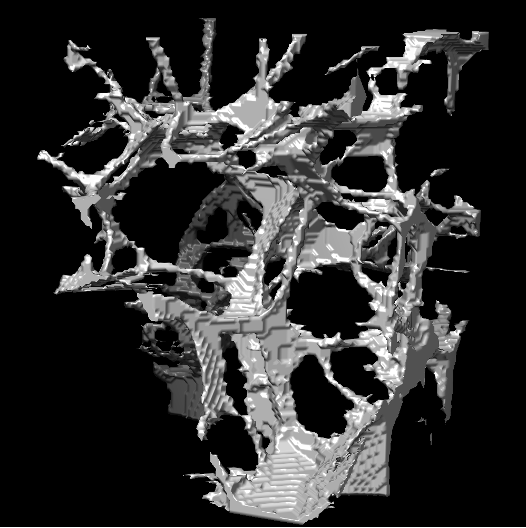
\includegraphics[width=\linewidth]{images/small_chunk.png}
        \small (a) Input subvolume.
    \end{minipage}\hfill
    \begin{minipage}[t]{0.31\textwidth}
        \centering
        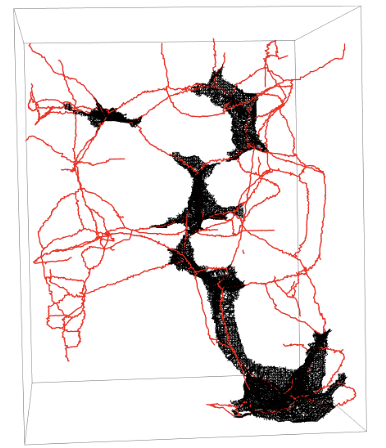
\includegraphics[width=\linewidth]{images/ambiguous_region.png}
        \small (b) Ambiguous regions.
    \end{minipage}\hfill
    \begin{minipage}[t]{0.31\textwidth}
        \centering
        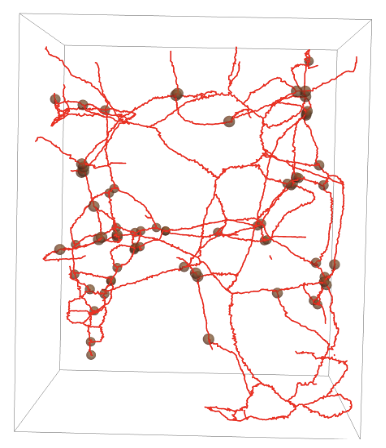
\includegraphics[width=\linewidth]{images/basic_junctions.png}
        \small (c) Retained candidates.
    \end{minipage}
    \caption{Candidate-junction extraction after ambiguous-region filtering.}
    \label{fig:filtering}
\end{figure}

\subsection{Merging touching junctions}

Skeletonization may represent one physical junction as several nearby graph vertices. Each candidate is associated with a maximal inscribed sphere whose center is the skeleton vertex and whose radius approximates local junction size. Let candidates $A$ and $B$ have center distance $d$ and radii $r_A$ and $r_B$. Define

\begin{equation}
    S_d(A,B)=\frac{d-r_A-r_B}{2\min(r_A,r_B)}.
    \label{eq:distance-score}
\end{equation}

The numerator approximates the gap between the two spheres, and the denominator normalizes that gap by the diameter of the smaller sphere. Thus $S_d\leq0$ indicates overlapping or touching spheres, while $S_d=1$ corresponds to a gap equal to the smaller diameter. The implementation treats $S_d\leq1$ as a necessary merging condition, motivated by the geometric criterion used to distinguish tubules from nodes in prior melt-network analysis \cite{skemerMelt}.

For clusters of candidates, the implementation evaluates connected cross-cluster pairs and retains the worst distance score. It also computes an angular-consistency score from incident skeleton branches. If the prospective merged junction has degree $k$, the combined score is

\begin{equation}
    S_{\mathrm{merge}}=\frac{k-1}{k}S_d+\frac{1}{k}S_a,
    \label{eq:merge-score}
\end{equation}

where $S_a$ is the angular score. A candidate cluster pair is eligible only when both $S_d\leq1$ and $S_{\mathrm{merge}}\leq1$. Eligible pairs are processed in ascending score order, and graph connectivity and degrees are updated after each merge.

\begin{algorithm}[htbp]
\caption{Merge touching junctions}
\KwIn{Candidate junctions $J$, initial skeleton graph $G_0$, current graph $G$}
\KwOut{Merged junction set and updated graph}
\While{an eligible connected cluster pair exists}{
    evaluate distance and angular scores for connected pairs\;
    sort eligible pairs by combined merge score\;
    merge the best available pair\;
    update cluster membership, graph edges, and junction degrees\;
}
\end{algorithm}

\section{Evaluation}

\subsection{Data and metric}

The method was evaluated on the full $500^3$ \dataset{} volume and on a $112\times118\times142$ subvolume. The subvolume was manually labeled by the author to provide a same-region reference distribution. A previously available distribution produced by the method associated with Zhu et al. \cite{sotamethod} came from an unidentified $250^3$ subvolume. Because that region is not spatially matched to either evaluation volume, it is included only as historical context and cannot support a controlled head-to-head accuracy claim.

For two normalized CN histograms $h^{(1)}$ and $h^{(2)}$, the reported discrepancy is the sum of squared errors over CN values 1 through 8:

\begin{equation}
    \operatorname{SSE}\!\left(h^{(1)},h^{(2)}\right)
    =\sum_{i=1}^{8}\left(h_i^{(1)}-h_i^{(2)}\right)^2.
    \label{eq:sse}
\end{equation}

Smaller values indicate more similar distributions.

\subsection{Results}

\begin{figure}[htbp]
    \centering
    \begin{minipage}[t]{0.48\textwidth}
        \centering
        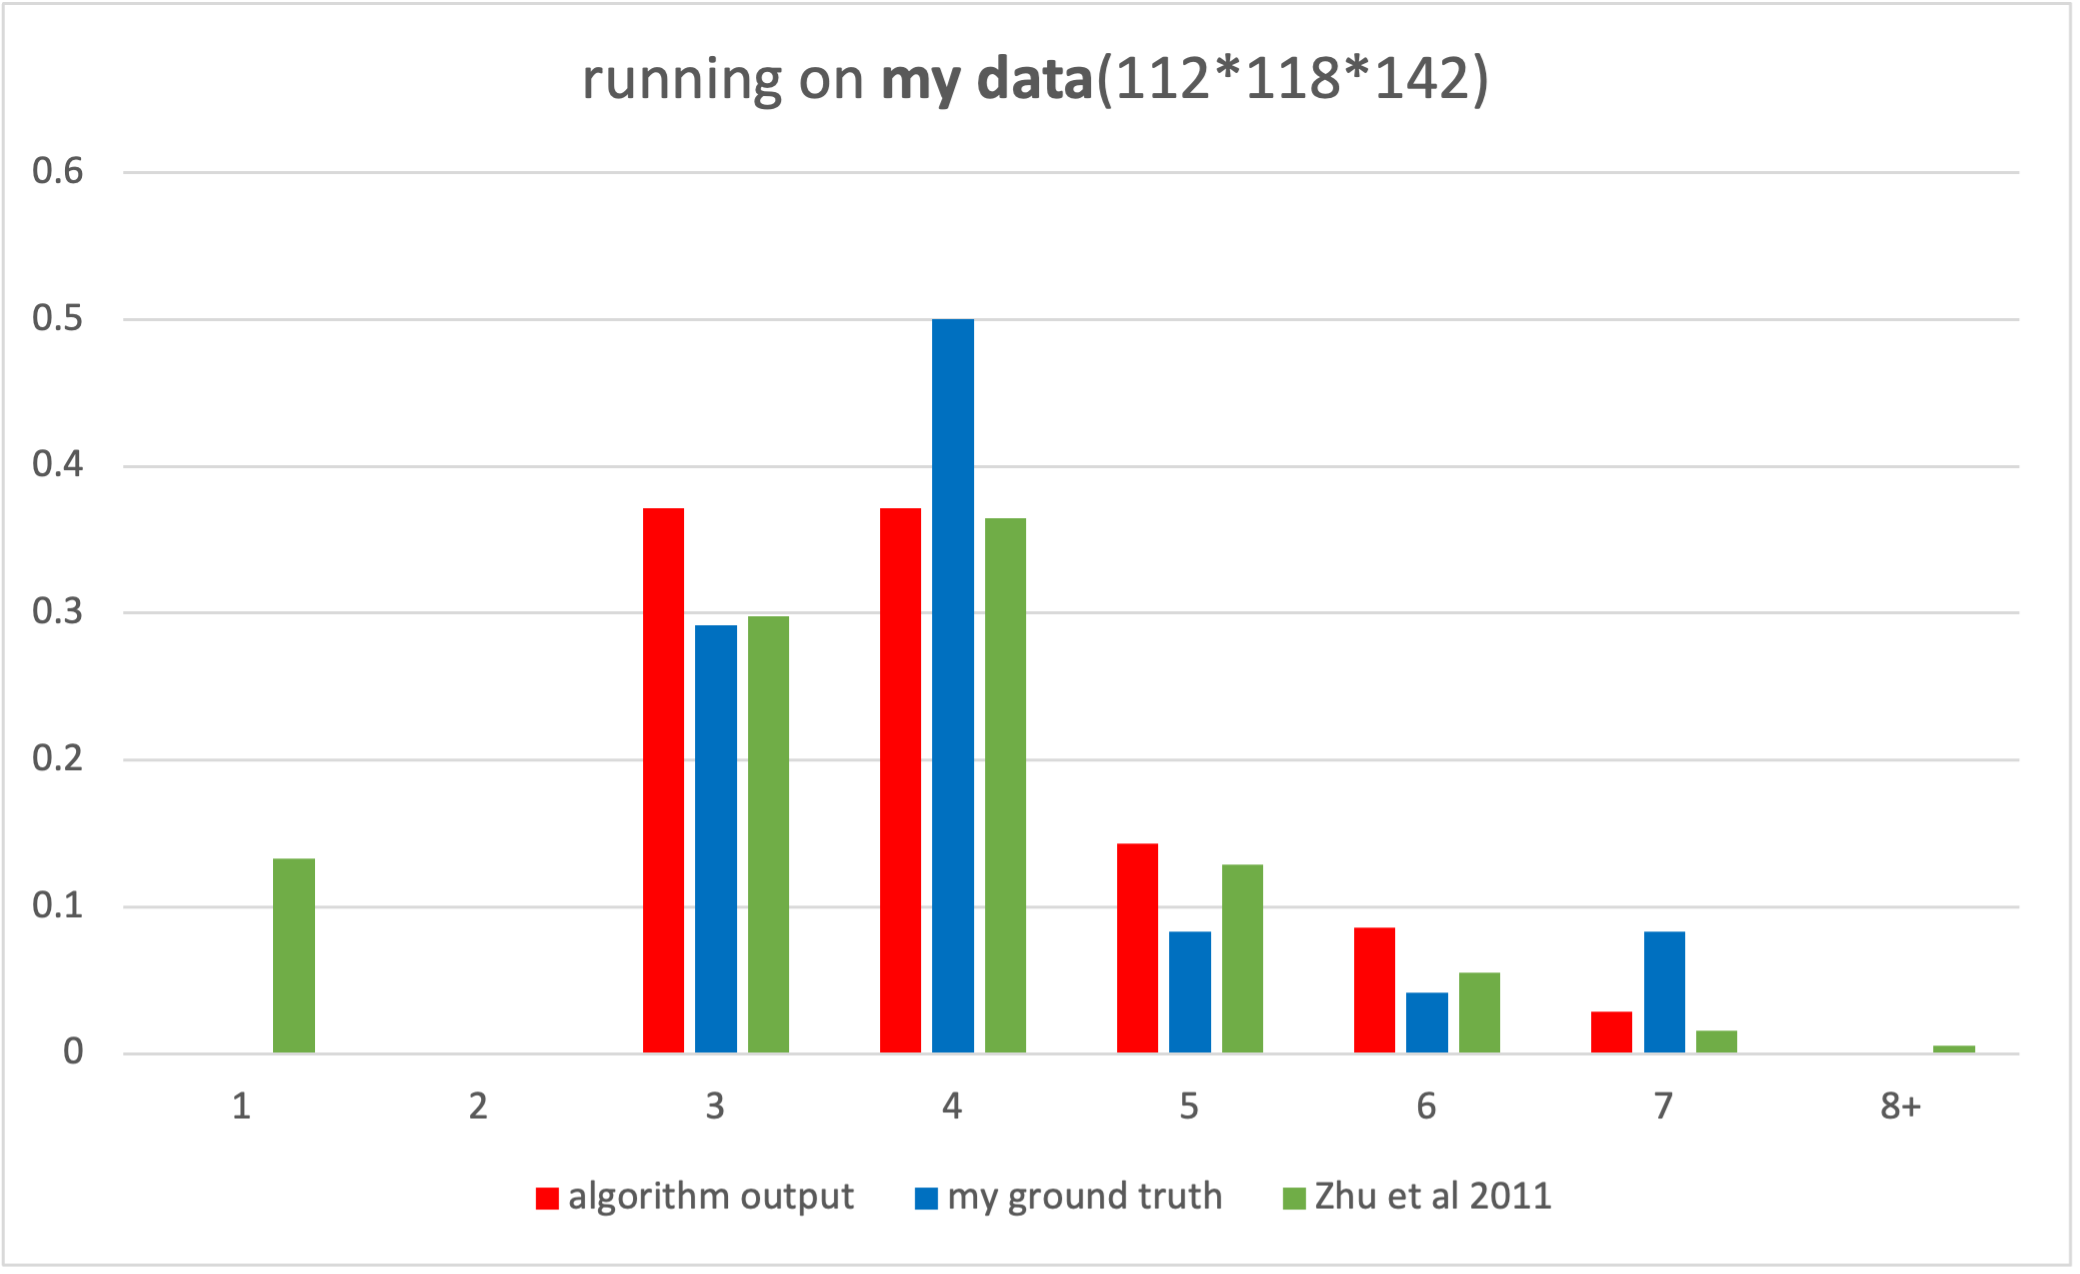
\includegraphics[width=\linewidth]{images/result1.png}
        \small (a) Proposed method and manual labels on the same subvolume; the unmatched historical distribution is shown only for context.
    \end{minipage}\hfill
    \begin{minipage}[t]{0.48\textwidth}
        \centering
        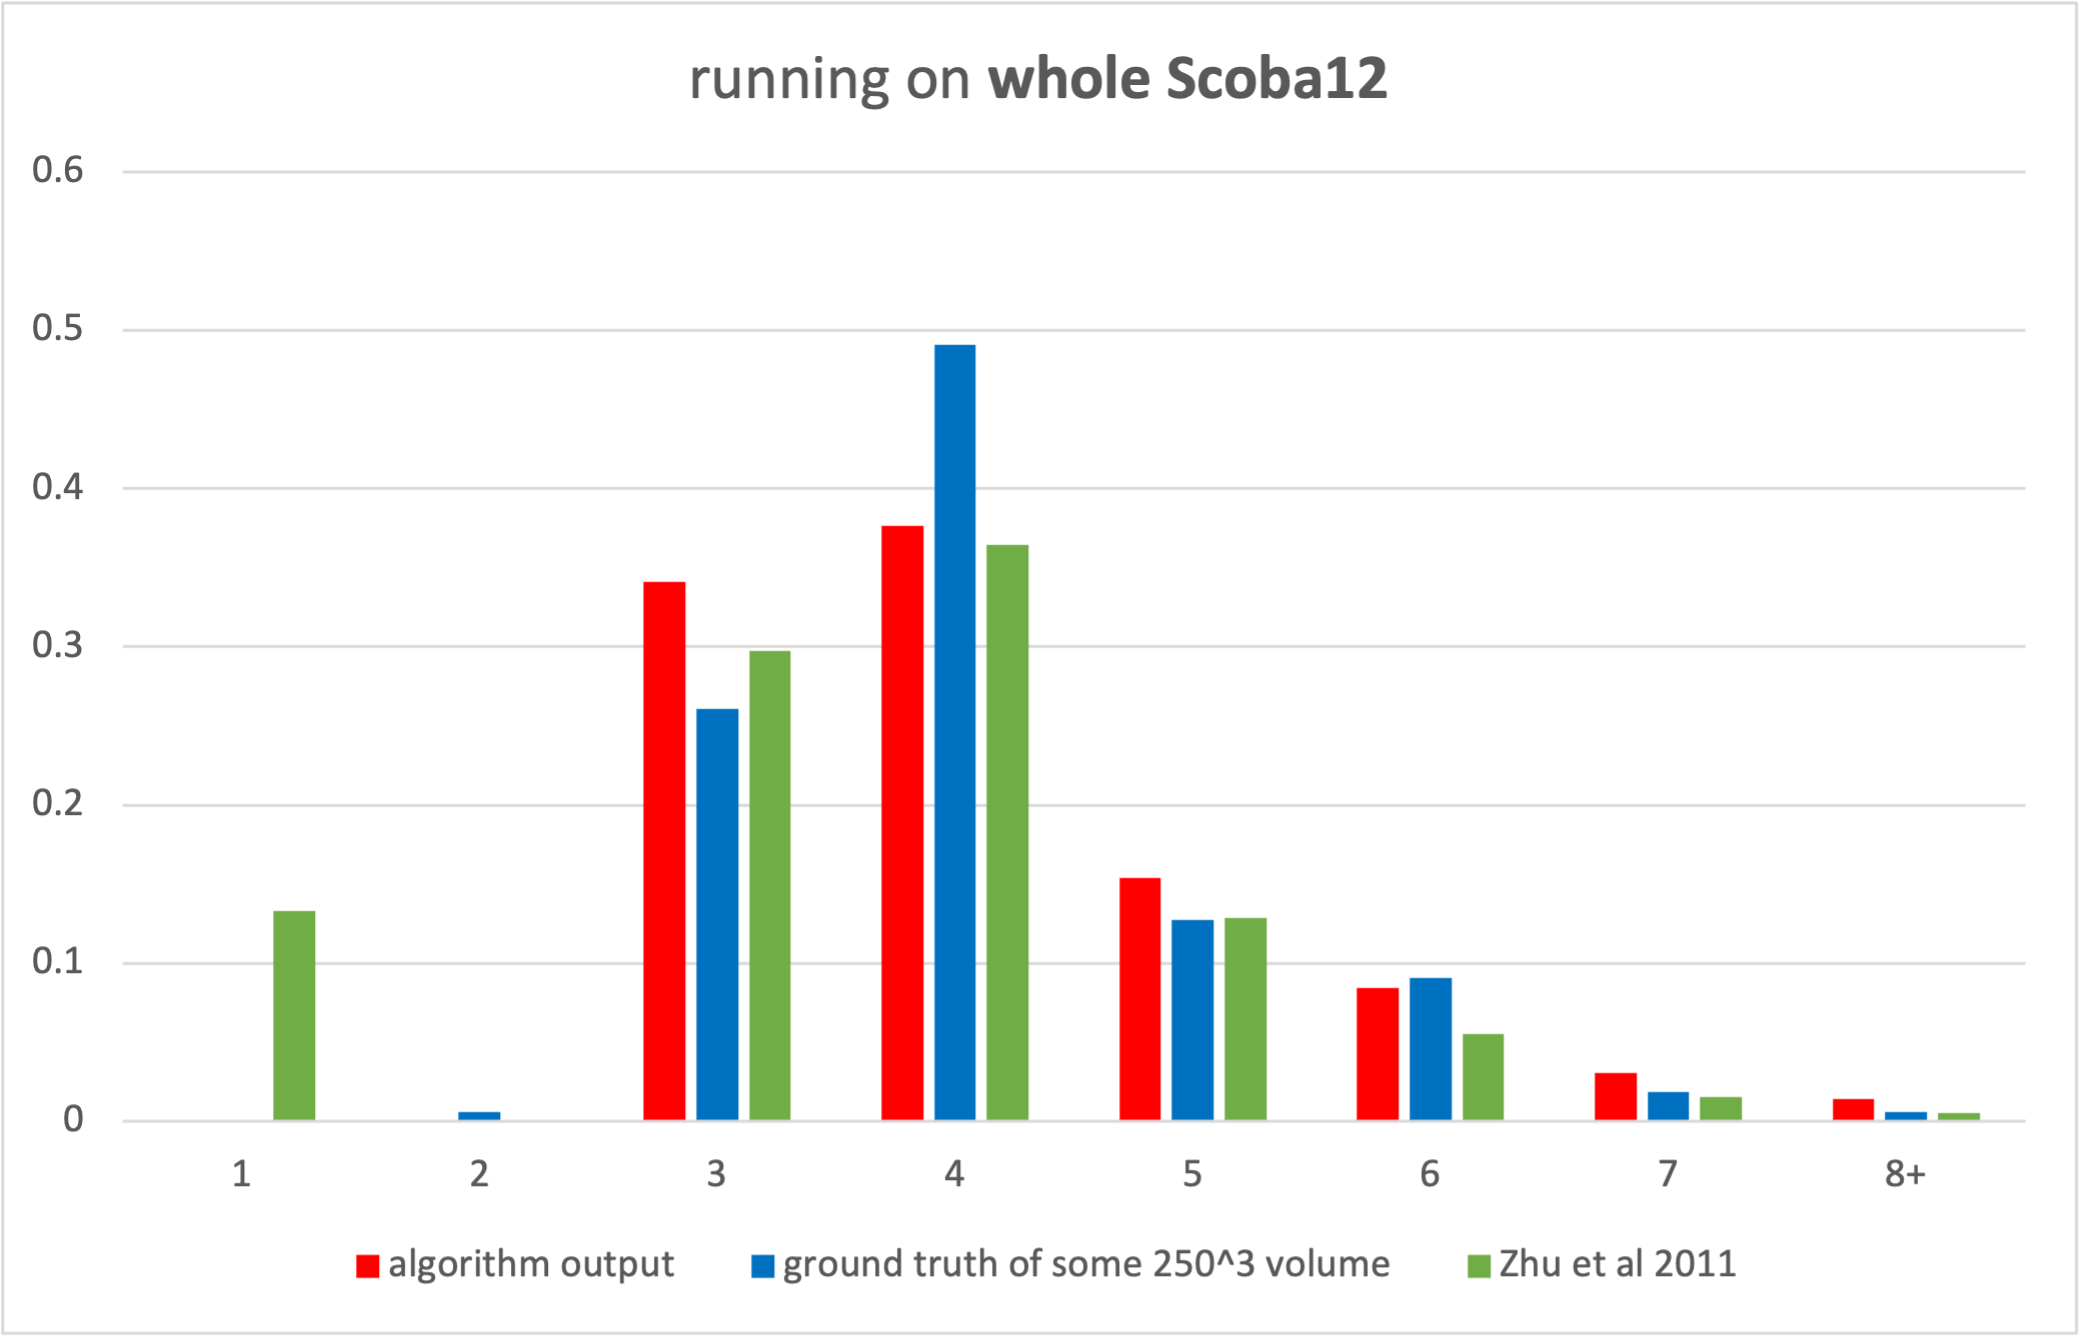
\includegraphics[width=\linewidth]{images/result2.png}
        \small (b) Full-volume output compared with the available reference distributions.
    \end{minipage}
    \caption{Coordination-number distributions used in the original project evaluation.}
    \label{fig:results}
\end{figure}

On the manually labeled $112\times118\times142$ subvolume, the proposed method obtained an SSE of $0.03137$. The unmatched historical $250^3$ distribution had an SSE of $0.03624$ relative to those labels. On the full-volume comparison shown in Figure~\ref{fig:results}(b), the corresponding values were $0.02063$ for the proposed method and $0.01864$ for the unmatched historical distribution.

These numbers should not be interpreted as evidence that either automated method is more accurate overall. The only same-region comparison available here is between the proposed method and the author's manual labels on the small subvolume. The broader evidence suggests that the pipeline captures the overall distribution shape, but it systematically overcounts CN~$=3$ and undercounts CN~$=4$.

\section{Failure Analysis}

\subsection{Spurious short branches}

Boundary roughness can create short skeleton branches that do not correspond to physical tubules. Each additional branch raises a vertex degree and can create a false CN~$=3$ junction.

\begin{figure}[htbp]
    \centering
    \begin{minipage}[t]{0.48\textwidth}
        \centering
        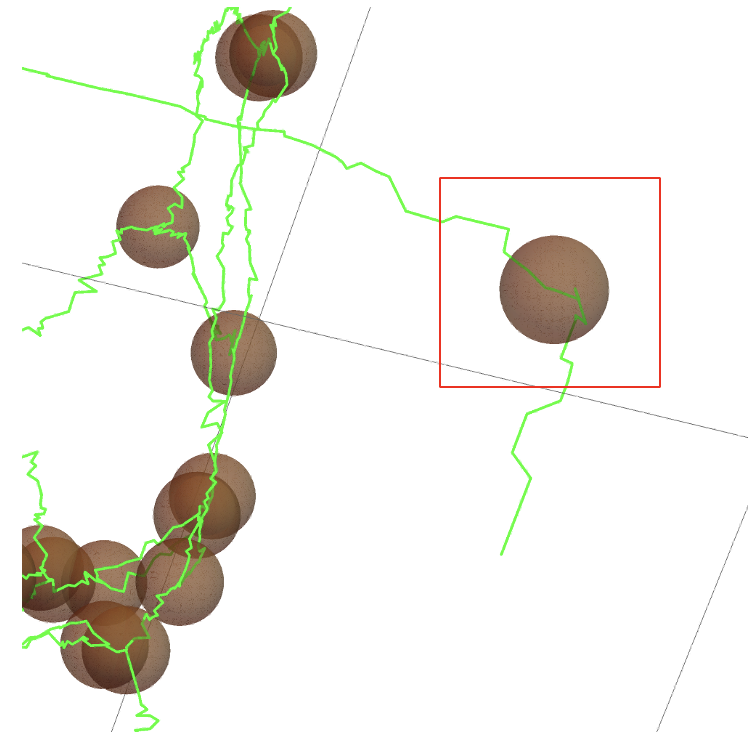
\includegraphics[width=\linewidth]{images/tiny_branch.png}
        \small (a) Skeleton with a short branch.
    \end{minipage}\hfill
    \begin{minipage}[t]{0.48\textwidth}
        \centering
        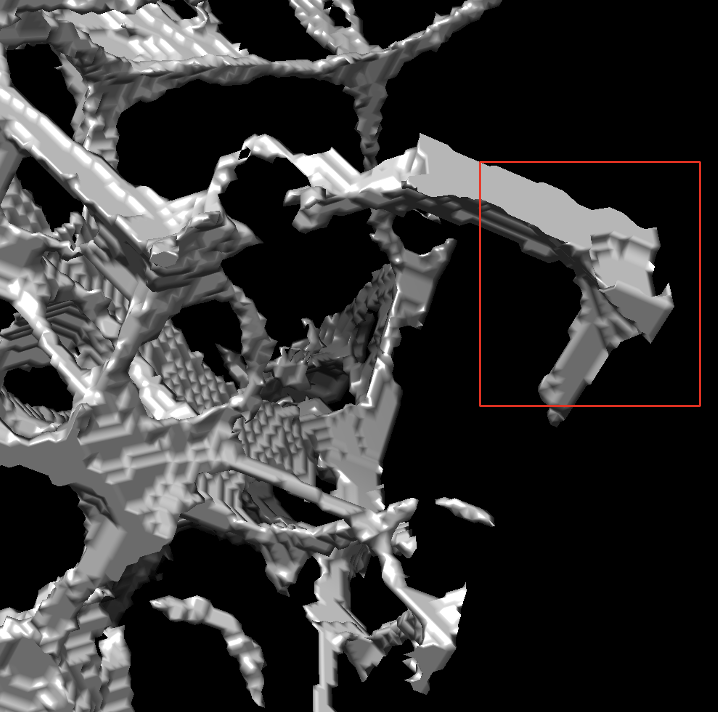
\includegraphics[width=\linewidth]{images/original_tiny_branch.png}
        \small (b) Corresponding volume region.
    \end{minipage}
    \caption{A short branch induced by surface roughness creates a false junction.}
    \label{fig:short-branch}
\end{figure}

\subsection{Crop-boundary artifacts}

Cropping a large volume can cut through a junction and create a flat, artificial boundary. The remaining shape may then be skeletonized as one or more ordinary junctions even though it should be excluded from the distribution. This effect also tends to inflate CN~$=3$.

\begin{figure}[htbp]
    \centering
    \begin{minipage}[t]{0.48\textwidth}
        \centering
        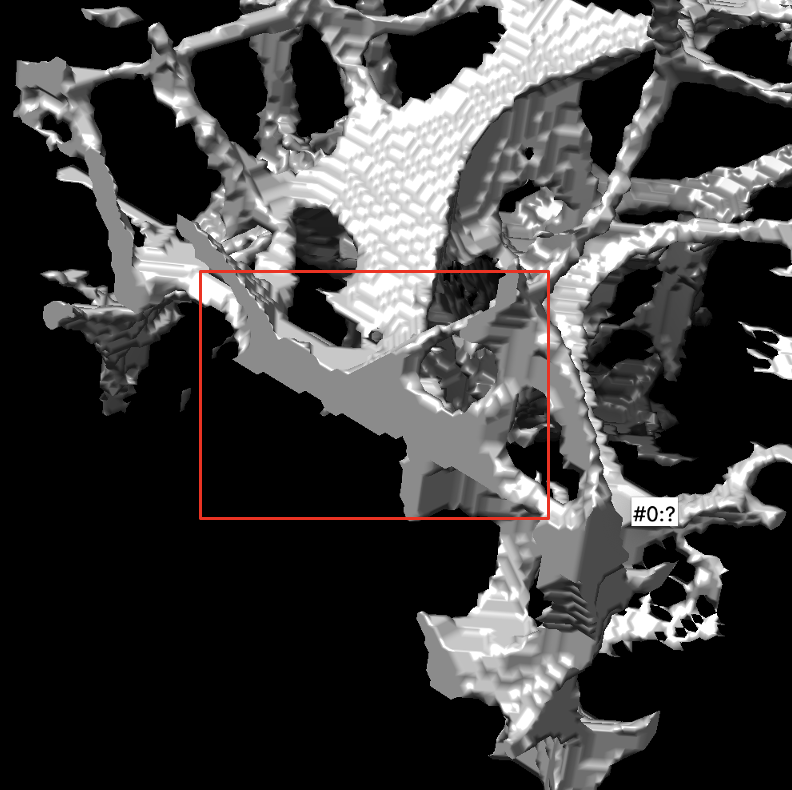
\includegraphics[width=\linewidth]{images/cutting_edge.png}
        \small (a) Shape truncated by the crop boundary.
    \end{minipage}\hfill
    \begin{minipage}[t]{0.48\textwidth}
        \centering
        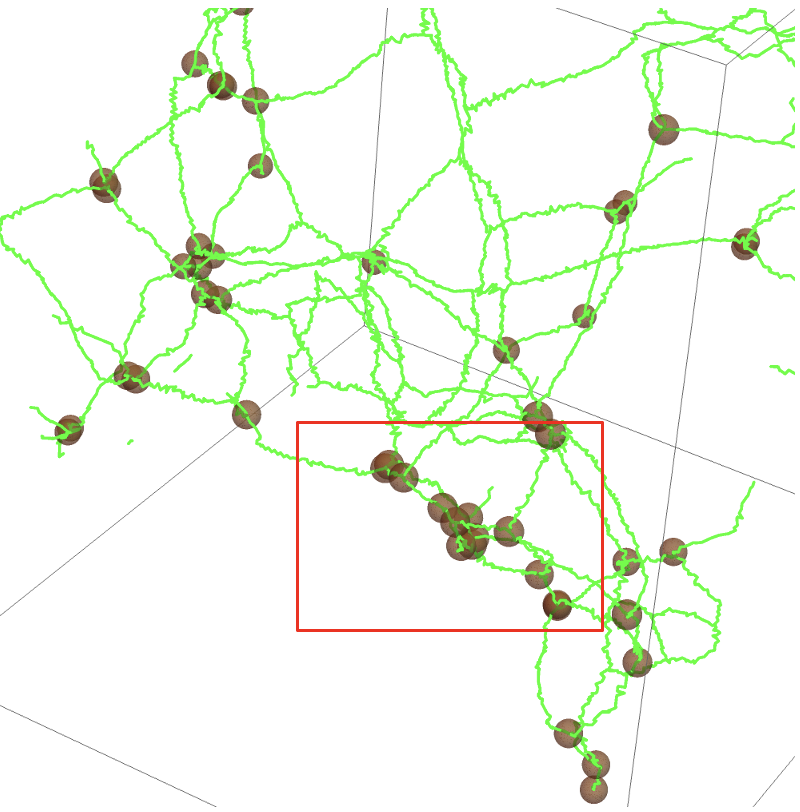
\includegraphics[width=\linewidth]{images/junctions_cutting_edge.png}
        \small (b) False junctions detected near the boundary.
    \end{minipage}
    \caption{Crop-boundary artifacts can be mistaken for physical junctions.}
    \label{fig:crop-artifact}
\end{figure}

\subsection{All-or-nothing removal of sheet regions}

The pipeline discards every candidate inside a detected sheet-like region. A more faithful treatment would remove the interior of the sheet while preserving its boundary and the tubules incident to that boundary. Their intersections can form valid junctions, often with CN~$=4$. Removing the entire region therefore helps explain the observed undercount of CN~$=4$.

\begin{figure}[htbp]
    \centering
    \begin{minipage}[t]{0.31\textwidth}
        \centering
        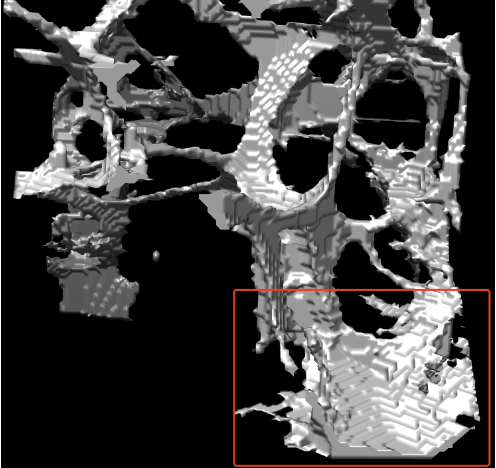
\includegraphics[width=\linewidth]{images/sheet.png}
        \small (a) Original sheet-like region.
    \end{minipage}\hfill
    \begin{minipage}[t]{0.31\textwidth}
        \centering
        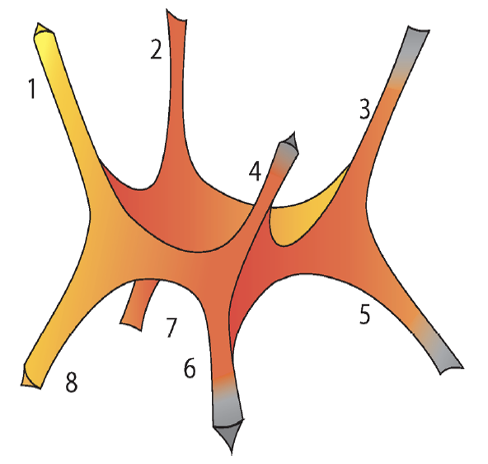
\includegraphics[width=\linewidth]{images/false_sheet.png}
        \small (b) Entire region removed.
    \end{minipage}\hfill
    \begin{minipage}[t]{0.31\textwidth}
        \centering
        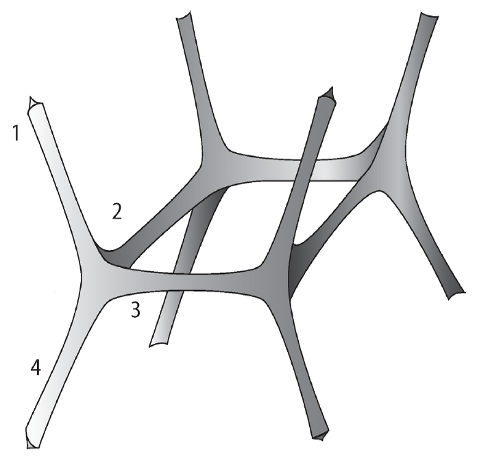
\includegraphics[width=\linewidth]{images/correct_sheet.png}
        \small (c) Desired boundary-preserving treatment.
    \end{minipage}
    \caption{A boundary-preserving sheet transformation would retain valid incident junctions.}
    \label{fig:sheet-processing}
\end{figure}

\section{Limitations and Future Work}

The available evaluation is preliminary. Its main limitations are:
\begin{itemize}
    \item The manual reference was produced by one annotator on one subvolume; inter-annotator agreement was not measured.
    \item The historical baseline distribution came from an unidentified, spatially unmatched region, so it is not a controlled baseline.
    \item Histogram SSE does not reveal which individual junctions were detected, missed, or assigned the wrong CN.
    \item Runtime, peak memory, and sensitivity to preprocessing and merge thresholds were not systematically measured.
\end{itemize}

The next evaluation should use matched volumes with independently reviewed junction annotations. It should report junction-level precision and recall, CN classification accuracy, distribution error, runtime, and peak memory. Algorithmically, the clearest next steps are short-branch pruning, explicit crop-boundary rejection, boundary-preserving processing of sheet regions, and a parameter-sensitivity study for dilation and merge thresholds.

\section{Conclusion}

This project demonstrates an end-to-end geometry-processing pipeline for estimating coordination-number distributions from three-dimensional melt-network volumes. The method combines morphological preprocessing and robust skeleton extraction with project-specific graph construction, ambiguous-region filtering, and geometry-aware merging of junction candidates. The results show that automated topology estimation is feasible, while the observed CN~$=3$ overcount and CN~$=4$ undercount expose specific weaknesses in skeleton noise handling and ambiguous-region processing. Those failure modes also define a practical path toward a stronger, reproducible benchmark and a more accurate system.

\bibliographystyle{plain}
\bibliography{references}

\end{document}
